\clearpage
\section{研究内容与技术路线}

\textbf{\color{red}(用一段文字+图说明论文研究内容的设置情况,以及研究内容间的逻辑关系。逻辑关系可以是并列、先后,总分等)}

针对上述问题,本论文的工作分为如下几个方面,如\cref{fig_1}所示。首先研究XXX,在此基础上研究XXX,基于上述研究成果实现XXX。

\begin{figure}[h] \label{fig_1}
	\centering
	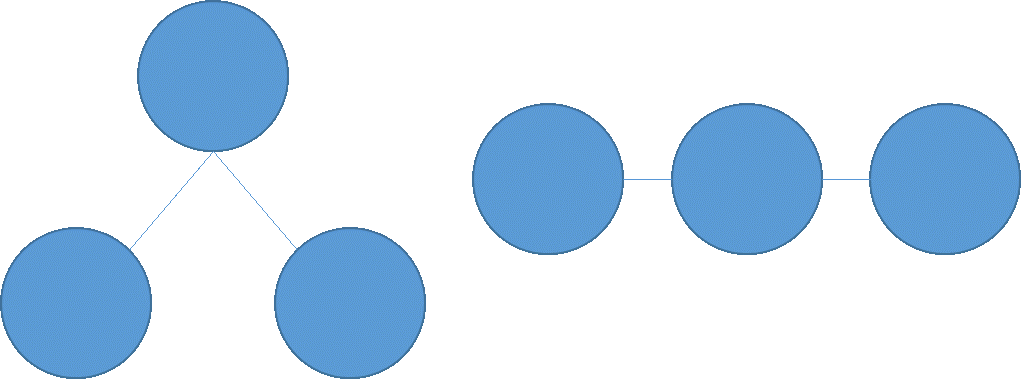
\includegraphics[width=0.4\linewidth]{fig_1.png}
	\caption{研究内容关系示意图}
\end{figure}

\textbf{\color{red}(下面分别介绍每个研究内容)}


\subsection{研究内容一:xxxxxxxxx}

\subsection{研究内容二:xxxxxxxxx}

\subsection{研究内容三:xxxxxxxxx}

\textbf{\color{red}(下面通过图文的形式说明论文技术方案)}

\subsection{XXXXX方法技术路线}

本文使用XXX方法技术路线。

\begin{figure}[h] \label{fig_2}
	\centering
	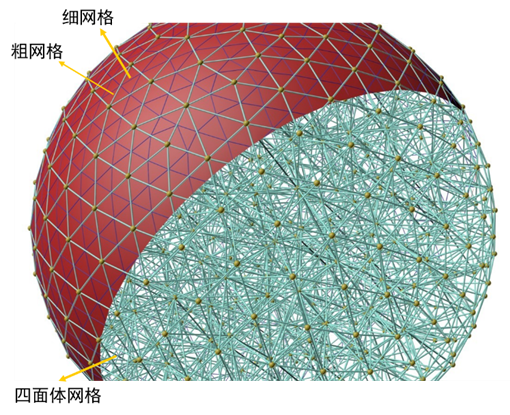
\includegraphics[width=0.6\linewidth]{fig_2.png}
	\caption{本论文拟构建的物理仿真模型示意图}
\end{figure}

\subsection{XXXXX方法技术路线}

\subsection{XXXXX方法技术路线}